\documentclass[12pt,a4paper]{article}

\usepackage[utf8]{inputenc}
\usepackage[T1]{fontenc}
\usepackage[slovene]{babel}
\usepackage{amsmath}
\usepackage{amssymb}
\usepackage{graphicx}
\usepackage{booktabs}
\usepackage{hyperref}
\usepackage{geometry}
\usepackage{enumitem}
\usepackage{microtype}

\geometry{margin=2.5cm}
\emergencystretch=2em
\graphicspath{{Pics/}{docs/Pics/}}
\hypersetup{hidelinks}

\title{Razširitev metode za analizo atrakcijskih bazenov z zaznavanjem platojev}
\author{Jure Hribar}
\date{\today}

\begin{document}

\maketitle

\begin{abstract}
Pri analizi dvodimenzionalnih optimizacijskih funkcij so atrakcijski bazeni uporaben način za prikaz območij, iz katerih lokalni spust vodi proti isti rešitvi oziroma lokalnemu optimumu. V ~\cite{jerebic_novel_2021} avtorji s pomočjo atrakcijskih bazenov definirajo nov način merjenja eksploracije in eksploatacije ExpBas(). Obstoječa implementacija omogočala izračun atrakcijskih bazenov, zaznavanje mej med njimi in barvanje posameznih bazenov. V tej nalogi je bila implementacija razširjena z zaznavanjem mej med atrakcijskimi bazeni in platoji, tj. povezanimi ravnimi območji z enako vrednostjo funkcije. Dodana je bila funkcija \texttt{detectPlateaus}, ki identificira platoje na diskretizirani mreži, jih označi z identifikatorji in izloči regije, ki so premajhne ali geometrijsko pretanke, da bi jih obravnavali kot prave platoje. Razširjen je bil tudi izris rezultatov, tako da je poleg slike atrakcijskih bazenov mogoče ustvariti še ločen prikaz zaznanih platojev. Dokument opisuje motivacijo, uporabljeno metodo, pričakovane rezultate in omejitve pristopa.
\end{abstract}

\section{Uvod}

Pri dvodimenzionalnih funkcijah lahko iskalni prostor diskretiziramo v mrežo točk, v vsaki točki izračunamo vrednost funkcije, poiščemo meje med atrakcijskimi bazeni ter nato z algoritmom barvanja določimo območja, ki pripadajo istemu atrakcijskemu bazenu~\cite{jerebic_novel_2021}. Tak prikaz razkrije število bazenov, njihove oblike in meje med njimi.

Obstoječa implementacija ni posebej obravnaval platojev. Vendar pri funkcijah s platoji nastopi dodaten primer: del funkcije je raven, zato več sosednjih točk zavzame enako vrednost funkcije. Takšna območja so pomembna, ker vplivajo na obnašanje optimizacijskih algoritmov. Na platoju gradient oziroma lokalna smer izboljšanja ni informativna, zato lahko algoritmi tam zastanejo, se premikajo naključno ali potrebujejo dodatna pravila za nadaljevanje iskanja.

Cilj naloge je bil razširiti obstoječo analizo tako, da sistem poleg meja med atrakcijskimi bazeni zazna tudi meje med bazeni in platoji. Za vsako točko mreže naj vemo kateremu atrakcijskemu bazenu pripada ali kateremu platoju.

Platoji so lahko koristni predvsem zato, ker pokažejo dele iskalnega prostora, kjer funkcijska vrednost ne daje več jasne informacije o smeri izboljšanja. To je pomembno pri interpretaciji optimizacijskih algoritmov na primer, če algoritem pride na plato, lahko veliko premikov izgleda enako dobrih.

Pri optimizacijskih problemih z omejitvami lahko omejitve ustvarijo območja, kjer je veliko točk enako kaznovanih ali imajo podobno vrednost kazenske funkcije. Če se kršitve omejitev pretvorijo v kazensko funkcijo, lahko nastanejo “ravne” ali skoraj ravne regije, kjer vse rešitve dobijo enako kazen. Zaznavanje platojev bi zato lahko pomagalo razumeti, ali algoritem raziskuje rob dopustnega območja, se zatakne v nedopustni regiji, ali pa se premika po območju, kjer ga penalizacija ne vodi več dovolj informativno.

\section{Metode}

\subsection{Vhodni podatki in diskretizacija}

Analiza temelji na dvodimenzionalni toplotni karti funkcije. Iskalni prostor je diskretiziran v pravokotno mrežo
\[
G = \{(i,j) \mid 0 \le i < n,\; 0 \le j < m\},
\]
kjer vsaka celica vsebuje koordinati \((x_1,x_2)\), vrednost funkcije \(f(x_1,x_2)\), identifikator atrakcijskega bazena in identifikator platoja. V implementaciji je to predstavljeno z razredom \texttt{Point}, ki hrani vrednosti \texttt{x1}, \texttt{x2}, \texttt{f}, \texttt{color} in \texttt{plateau}.

Toplotna karta se prebere iz stisnjenega objekta \texttt{HeatMap2D}. Razred \texttt{Fill2D} nato nad mrežo izvede označevanje mej, barvanje atrakcijskih bazenov in zaznavanje platojev. Prag za minimalno velikost platoja je nastavljen s parametrom \texttt{minPlateauSize}, ki je definiran v konfiguracijski datoteki \texttt{config.properties}.

\subsection{Zaznavanje mej med bazeni in platoji}

Osnovna metoda za zaznavanje mej med bazeni je bila razširjena v delu kode, ki obravnava meje platojev (\texttt{makeBoundariesPlateau}). Prejšnji pristop je zaznaval predvsem lokalne vrhove oziroma točke, kjer je vrednost trenutne celice večja od vrednosti sosedov v vodoravni, navpični ali diagonalni smeri. Pri platojih pa meja pogosto nastane v vzorcu, kjer imata dve sosednji celici enako vrednost, naslednja celica pa je višja ali nižja.

Zato razširjeni algoritem v vodoravni in navpični smeri preverja vzorce oblike:
\[
a = b < c,\qquad a = b > c,\qquad a < b = c,\qquad a > b = c,\qquad a < b > c.
\]
Ti primeri pokrijejo prehode iz neravnega območja v ravno območje, iz ravnega območja v neravno območje in klasičen vrh med dvema nižjima sosedoma. Celice, ki ustrezajo tem pogojem, se označijo kot meja z vrednostjo \texttt{color = 0}. Na ta način kasnejši algoritem barvanja atrakcijskih bazenov ne poveže območij, ki jih mora ločiti meja platoja.

\subsection{Barvanje atrakcijskih bazenov}

Po označitvi mej se nad preostalimi celicami izvede barvanje povezanih komponent. Implementacija podpira pristopa \texttt{scanline} in \texttt{boundary}; v eksperimentalnem cevovodu se uporablja \texttt{scanline}. Vsaka nepobarvana celica, ki ni meja, se uporabi kot seme novega bazena. Algoritem nato razširi trenutno barvo po povezanem območju, dokler ne doseže mejnih celic.

Identifikator bazena je shranjen v polju \texttt{color}. Vrednost \texttt{0} pomeni mejo, pozitivne vrednosti pa predstavljajo posamezne atrakcijske bazene. Ta del ostaja osnova celotnega pristopa, saj zaznavanje platojev poteka šele po tem, ko so meje in bazeni že določeni.

\subsection{Identifikacija platojev}

Plato je v tej nalogi definiran kot povezana regija diskretne mreže, v kateri imajo vse celice enako vrednost funkcije in ki je dovolj velika ter dovolj široka, da ni le artefakt diskretizacije. Funkcija \texttt{detectPlateaus} zato išče povezane komponente celic z enako vrednostjo \(f\), pri čemer uporablja 4-sosedstvo:
\[
N_4(i,j)=\{(i-1,j),(i+1,j),(i,j-1),(i,j+1)\}.
\]

Algoritem poteka v naslednjih korakih:

\begin{enumerate}[label=\arabic*.]
    \item Preleti vse celice mreže.
    \item Za vsako še neobiskano celico, ki ni meja, izbere vrednost \texttt{seedF}.
    \item S skladom izvede poplavljanje po 4-sosedstvu in v trenutno regijo doda samo celice z enako vrednostjo funkcije \texttt{seedF}.
    \item Za najdeno regijo izračuna velikost notranjega jedra.
    \item Regijo označi kot plato samo, če je velikost jedra večja od \texttt{minPlateauSize}.
\end{enumerate}

Med izvajanjem se celice začasno označijo z vrednostjo \texttt{plateau = -1}. S tem se prepreči, da bi bila ista celica večkrat dodana na sklad. Regije, ki niso sprejete kot plato, dobijo vrednost \texttt{plateau = -2}; pozitivne vrednosti \texttt{plateau} pa predstavljajo identifikatorje zaznanih platojev.

\subsection{Izločanje majhnih pik in tankih črt}

Samo preverjanje števila celic v povezani regiji ni dovolj. Tanka ravna črta je lahko dolga in zato vsebuje veliko celic, vendar ne predstavlja pravega dvodimenzionalnega platoja. Zato algoritem ne uporablja neposredno velikosti celotne regije, temveč velikost njenega notranjega jedra.

Celica pripada jedru regije samo, če ima vse štiri ortogonalne sosede v isti regiji. Formalno je celica \((i,j)\) jedrna celica, če velja:
\[
(i-1,j), (i+1,j), (i,j-1), (i,j+1) \in R,
\]
kjer je \(R\) trenutno najdena povezana regija z enako vrednostjo funkcije. Celice na robu mreže in celice na robu regije zato niso del jedra.

Ta postopek deluje kot ena iteracija morfološke erozije. Posamezne pike, ozke strukture in črte debeline enega piksla nimajo notranjega jedra, zato so zavrnjene. Regija se sprejme kot plato samo, če velja:
\[
|core(R)| > \texttt{minPlateauSize}.
\]

\subsection{Pomnilniška učinkovitost}

Implementacija uporablja dve vnaprej alocirani celoštevilski tabeli: eno za sklad pri poplavljanju in eno za celice trenutne regije. Celica \((x,y)\) je zakodirana kot eno število
\[
cell = x \cdot m + y.
\]
S tem se izognemo ustvarjanju velikega števila objektov, kot so pari koordinat ali množice. Tak pristop je posebej pomemben pri visokih ločljivostih, na primer pri mrežah velikosti \(10000 \times 10000\), kjer bi objektne strukture povzročile zelo veliko porabo pomnilnika.

\subsection{Vizualizacija}

Razred \texttt{Measure} je bil razširjen tako, da poleg slike atrakcijskih bazenov ustvari še ločeno sliko platojev. V prvem izrisu so prikazani atrakcijski bazeni, pri čemer so meje obarvane črno. V drugem izrisu so meje prav tako črne, zaznani platoji pa dobijo ločene barve. Celice, ki ne pripadajo nobenemu platoju, so prikazane s svetlo sivo barvo. Slika platojev se shrani z imenom oblike
\[
\texttt{<ime\_problema>\_plateaus.png}.
\]

Za barvanje platojev se uporablja deterministično razporejanje odtenkov z zlatim razmerjem, kar zmanjša verjetnost, da bi sosednji platoji dobili vizualno preveč podobne barve. Izris vključuje tudi legendo z oznakami \texttt{P1}, \texttt{P2}, itd.

\section{Rezultati}

Razširitev omogoča, da sistem poleg običajnega prikaza atrakcijskih bazenov prikaže tudi prostorsko razporeditev platojev. To je posebej pomembno pri testnih funkcijah, ki vsebujejo eksplicitno ravna območja, in pri funkcijah, kjer lahko diskretizacija povzroči navidezno ravne regije. V nadaljevanju so prikazani rezultati za funkcije \texttt{InvertedHemispheres}, \texttt{SpherePlateau}, \texttt{RastriginPlateau}, \texttt{CosinePlateausSmooth}, \texttt{PiecewiseLinearPlateau} in \texttt{TanhRadialStep}.

Pri funkcijah s platoji pričakujemo, da bo nov algoritem:

\begin{itemize}
    \item zaznal povezane regije z enako vrednostjo funkcije,
    \item ločil platoje od okoliških atrakcijskih bazenov,
    \item izločil osamljene točke in majhne regije,
    \item zavrnil enopikselske ravne črte, ker nimajo notranjega jedra,
    \item ustvaril ločen slikovni prikaz samo za platoje.
\end{itemize}

V konfiguraciji je parameter \texttt{minPlateauSize} nastavljen na vrednost 5. To pomeni, da mora imeti kandidatna regija več kot pet jedrnih celic, da je označena kot plato. Višja vrednost parametra omogoča strožje filtriranje, nižja vrednost pa bolj občutljivo zaznavanje manjših platojev.

\subsection{\texttt{InvertedHemispheres}}

Funkcija \texttt{InvertedHemispheres} opisuje dve obrnjeni polkrogli oziroma dve vdolbini v sicer ravni osnovni ploskvi. Pri privzetih parametrih \(B=2\), \(a=2\) in \(r=1.7\) je definirana kot
\[
f(x,y)=B-\max\left(0,\sqrt{r^2-(x-a)^2-y^2},\sqrt{r^2-(x+a)^2-y^2}\right),
\]
pri čemer je posamezen koren upoštevan samo znotraj pripadajoče krožnice, zunaj nje pa prispeva vrednost 0. Funkcija ima dve simetrični vdolbini s središčema pri \((-a,0)\) in \((a,0)\), kar je razvidno iz slike~\ref{fig:inverted-plot}.

\begin{figure}[htbp]
\centering
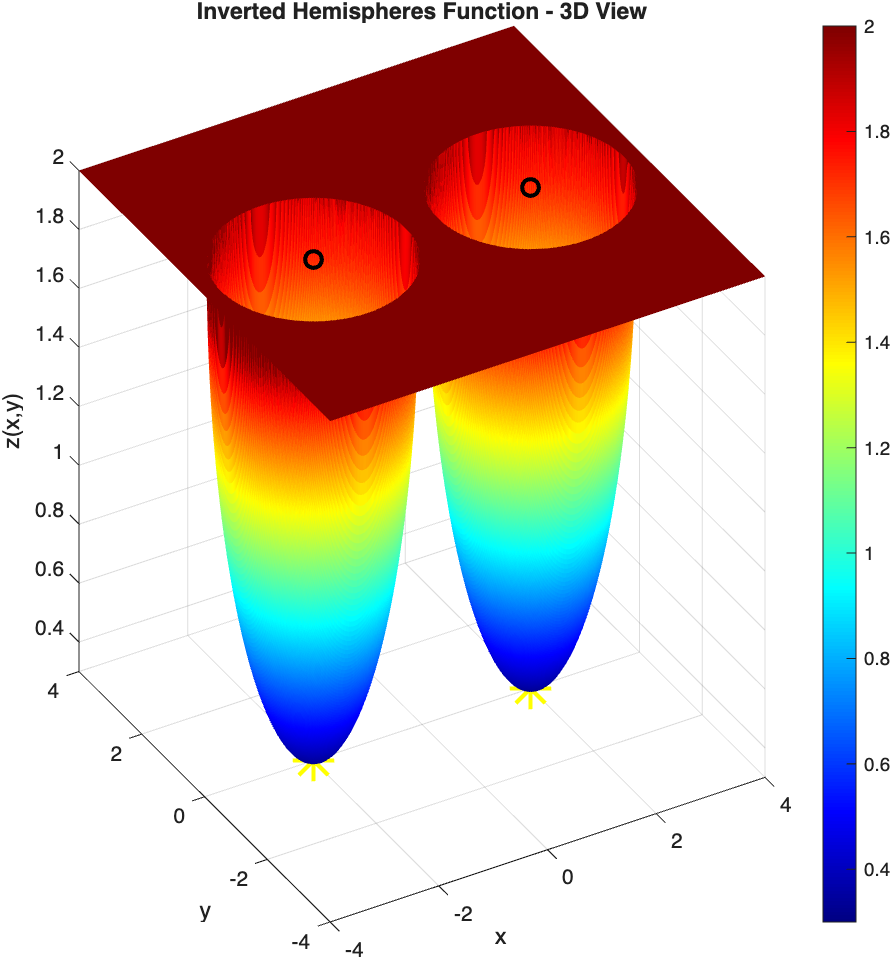
\includegraphics[width=0.78\textwidth]{InvertedHemispheresPlot.png}
\caption{Graf funkcije \texttt{InvertedHemispheres}. Vidni sta dve ločeni vdolbini v ravni osnovni ploskvi.}
\label{fig:inverted-plot}
\end{figure}

Na sliki~\ref{fig:inverted-basins} sta vidna dva glavna atrakcijska bazena, ki ustrezata obema vdolbinama. Črna meja označuje ločnico med območjema, iz katerih lokalno gibanje vodi v eno ali drugo minimumsko območje.

\begin{figure}[htbp]
\centering
\includegraphics[width=0.78\textwidth]{InvertedHemispheresBasins.png}
\caption{Atrakcijski bazeni funkcije \texttt{InvertedHemispheres}.}
\label{fig:inverted-basins}
\end{figure}

Slika~\ref{fig:inverted-plateaus} pokaže zaznane platoje. Ker je funkcija zunaj obeh vdolbin konstantna, algoritem zazna velik plato na ravnem zunanjem delu funkcije. To je primer pravega platoja, saj gre za povezano dvodimenzionalno območje z enako vrednostjo funkcije.

\begin{figure}[htbp]
\centering
\includegraphics[width=0.78\textwidth]{InvertedHemispheres_plateaus.png}
\caption{Zaznani platoji funkcije \texttt{InvertedHemispheres}.}
\label{fig:inverted-plateaus}
\end{figure}

\subsection{\texttt{SpherePlateau}}

Funkcija \texttt{SpherePlateau} je osnovana na sferični funkciji, vendar vsebuje križno oblikovan plato. V dveh dimenzijah je definirana kot
\[
f(x,y)=
\begin{cases}
144, & x\in[10,17]\ \text{ali}\ y\in[10,17],\\
x^2+y^2, & \text{sicer}.
\end{cases}
\]
Na sliki~\ref{fig:sphere-plot} je zato poleg klasične parabolične oblike vidno ravno območje, ki nastane, kadar ena izmed koordinat pade v interval \([10,17]\).

\begin{figure}[htbp]
\centering
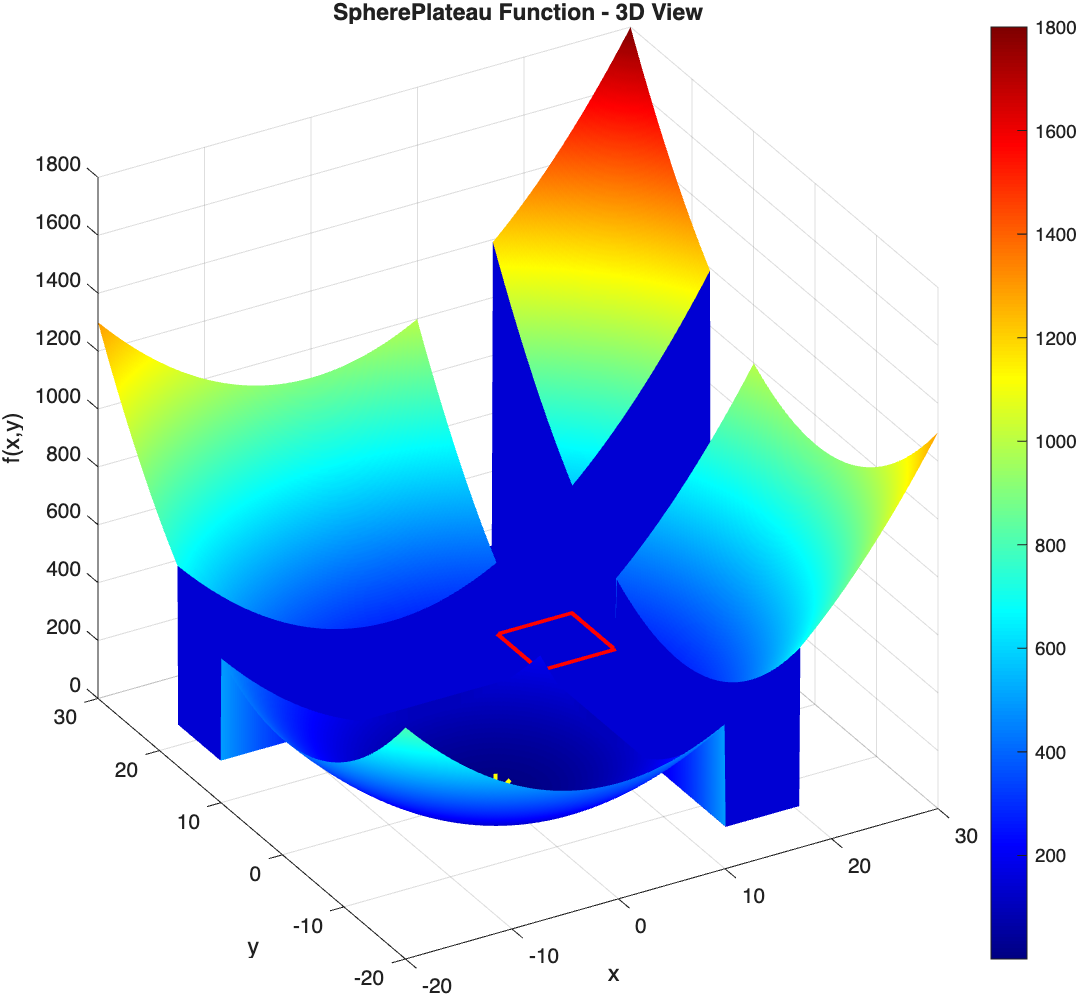
\includegraphics[width=0.78\textwidth]{SpherePlateauPlot.png}
\caption{Graf funkcije \texttt{SpherePlateau} s križno oblikovanim platojem.}
\label{fig:sphere-plot}
\end{figure}

Slika~\ref{fig:sphere-basins} prikazuje, da dodani plato vpliva na strukturo meja med atrakcijskimi bazeni. Meje se pojavijo tudi na prehodih med paraboličnim delom funkcije in ravnim območjem.

\begin{figure}[htbp]
\centering
\includegraphics[width=0.78\textwidth]{SpherePlateauBasins.png}
\caption{Atrakcijski bazeni funkcije \texttt{SpherePlateau}.}
\label{fig:sphere-basins}
\end{figure}

Na sliki~\ref{fig:sphere-plateaus} je plato jasno ločen od ostalega prostora. Ker gre za široko regijo z notranjim jedrom, ga filter \texttt{minPlateauSize} sprejme kot pravi plato.

\begin{figure}[htbp]
\centering
\includegraphics[width=0.78\textwidth]{SpherePlateau_plateaus.png}
\caption{Zaznani platoji funkcije \texttt{SpherePlateau}.}
\label{fig:sphere-plateaus}
\end{figure}

\subsection{\texttt{RastriginPlateau}}

Funkcija \texttt{RastriginPlateau} izhaja iz dvodimenzionalne Rastriginove funkcije
\[
g(x,y)=20+x^2+y^2-10\cos(2\pi x)-10\cos(2\pi y).
\]
Okoli lokalnih minimumov pri celoštevilskih koordinatah in okoli lokalnih maksimumov pri polceloštevilskih koordinatah so dodani majhni kvadratni platoji. Pri privzeti širini platoja \(s=0.1\) velja
\[
f(x,y)=
\begin{cases}
g(\operatorname{round}(x),\operatorname{round}(y)), & |x-\operatorname{round}(x)|\le s/2\ \land\ |y-\operatorname{round}(y)|\le s/2,\\
g(\lfloor x\rfloor+0.5,\lfloor y\rfloor+0.5), & |x-(\lfloor x\rfloor+0.5)|\le s/2\ \land\ |y-(\lfloor y\rfloor+0.5)|\le s/2,\\
g(x,y), & \text{sicer}.
\end{cases}
\]
Slika~\ref{fig:rastrigin-plot} prikazuje večmodalno strukturo funkcije, kjer se majhni platoji pojavijo v okolici ekstremov.

\begin{figure}[htbp]
\centering
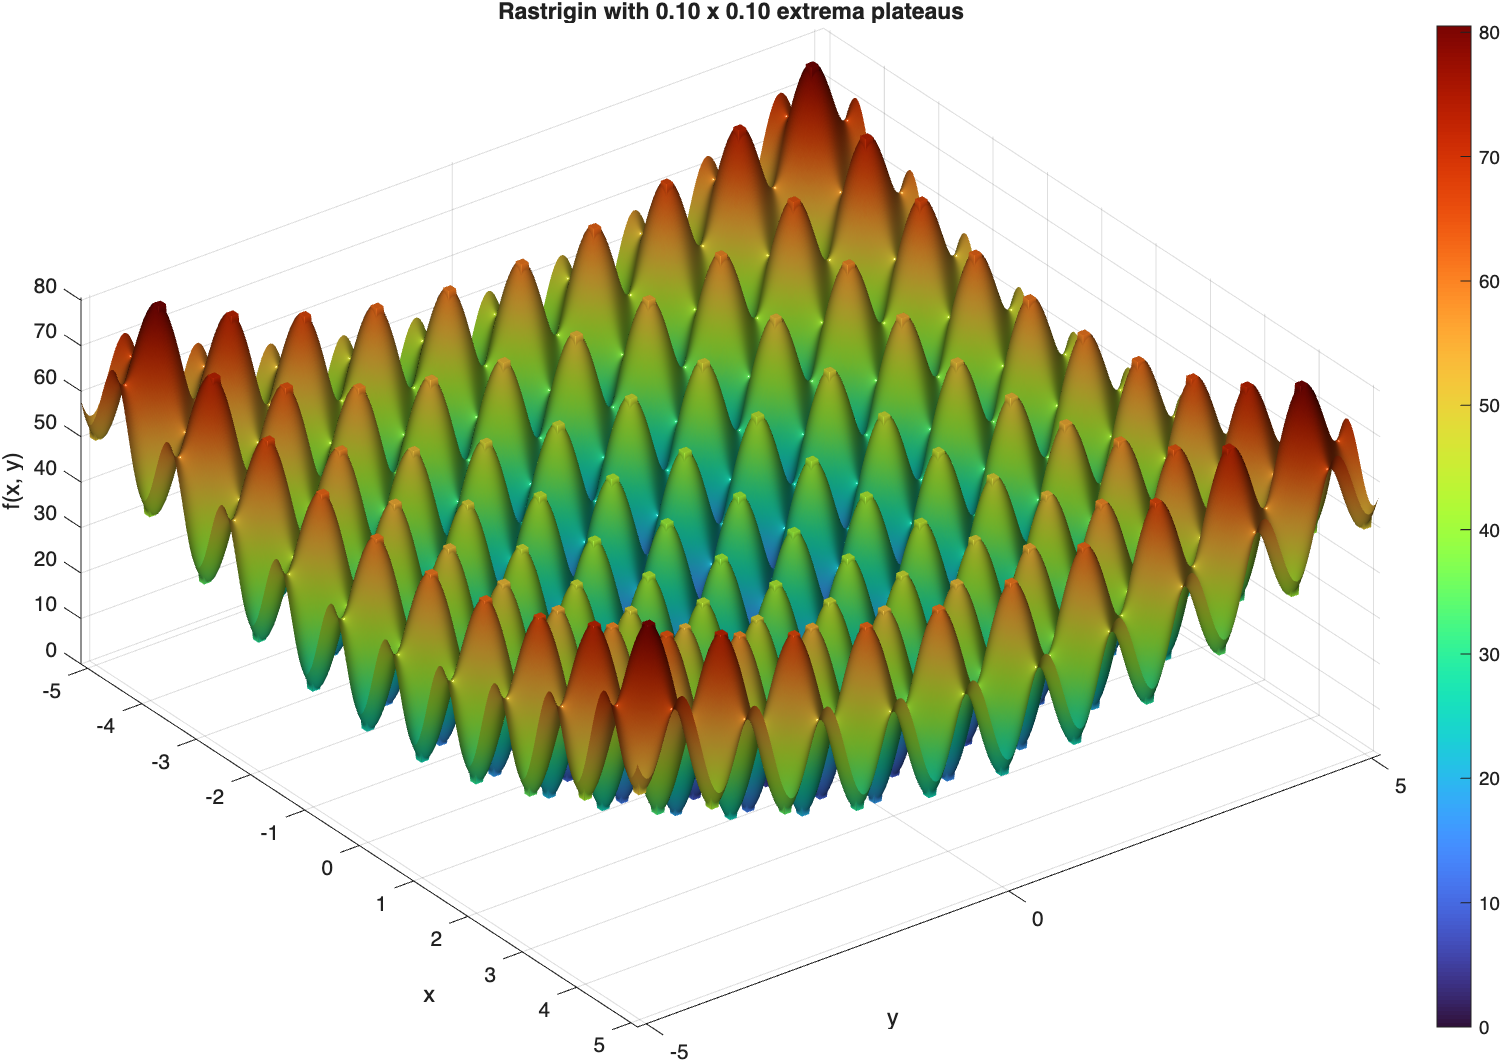
\includegraphics[width=0.78\textwidth]{RastriginPlateauPlot.png}
\caption{Graf funkcije \texttt{RastriginPlateau}.}
\label{fig:rastrigin-plot}
\end{figure}

Na sliki~\ref{fig:rastrigin-basins} je razvidna razdrobljena struktura atrakcijskih bazenov, značilna za Rastriginovo funkcijo. Dodani platoji predstavljajo majhne ravne regije znotraj sicer oscilatorne površine.

\begin{figure}[htbp]
\centering
\includegraphics[width=0.78\textwidth]{RastriginPlateauBasins.png}
\caption{Atrakcijski bazeni funkcije \texttt{RastriginPlateau}.}
\label{fig:rastrigin-basins}
\end{figure}

Slika~\ref{fig:rastrigin-plateaus} pokaže, kateri izmed teh ravnih območij so po kriteriju notranjega jedra prepoznani kot platoji. Ker so platoji majhni, je njihova zaznava posebej odvisna od ločljivosti mreže in parametra \texttt{minPlateauSize}.

\begin{figure}[htbp]
\centering
\includegraphics[width=0.78\textwidth]{RastriginPlateau_plateaus.png}
\caption{Zaznani platoji funkcije \texttt{RastriginPlateau}.}
\label{fig:rastrigin-plateaus}
\end{figure}

\subsection{\texttt{CosinePlateausSmooth}}

Funkcija \texttt{CosinePlateausSmooth} uporablja osnovo
\[
g(x,y)=\cos(x)\cos(y),
\]
platoje pa tvori z odrezom pri pragu \(c\). Pri privzeti vrednosti \(c=0.9\) je
\[
f(x,y)=\min(\cos(x)\cos(y),c).
\]
Platoji zato nastanejo okoli vrhov kosinusne površine, meja platoja pa sledi nivojnici \(g(x,y)=c\). Slika~\ref{fig:cosine-plot} prikazuje gladko periodično strukturo s sploščenimi vrhovi.

\begin{figure}[htbp]
\centering
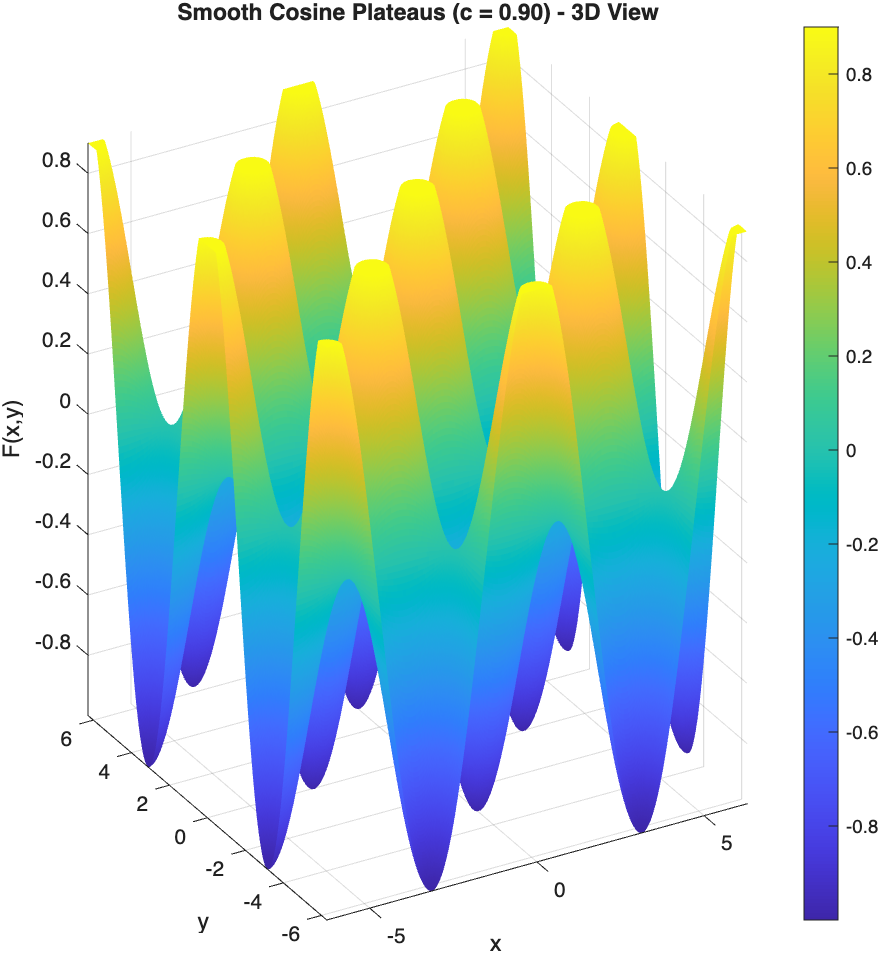
\includegraphics[width=0.78\textwidth]{CosinePlateauSmoothPlot.png}
\caption{Graf funkcije \texttt{CosinePlateausSmooth}.}
\label{fig:cosine-plot}
\end{figure}

Na sliki~\ref{fig:cosine-basins} so vidna periodično razporejena območja atrakcije. Ker so platoji ustvarjeni okoli vrhov, njihove meje vplivajo na delitev prostora v okolici ponavljajočih se struktur.

\begin{figure}[htbp]
\centering
\includegraphics[width=0.78\textwidth]{CosinePlateausSmooth.png}
\caption{Atrakcijski bazeni funkcije \texttt{CosinePlateausSmooth}.}
\label{fig:cosine-basins}
\end{figure}

Slika~\ref{fig:cosine-plateaus} prikazuje zaznane platoje. Pri domeni \([-2\pi,2\pi]^2\) pričakujemo več ločenih platojskih regij, ki ustrezajo sploščenim vrhovom kosinusne funkcije.

\begin{figure}[htbp]
\centering
\includegraphics[width=0.78\textwidth]{CosinePlateausSmooth_plateaus.png}
\caption{Zaznani platoji funkcije \texttt{CosinePlateausSmooth}.}
\label{fig:cosine-plateaus}
\end{figure}

\subsection{\texttt{PiecewiseLinearPlateau}}

Funkcija \texttt{PiecewiseLinearPlateau} je kosovno linearna funkcija s kvadratnim platojem na območju \([3,5]\times[3,5]\). Njena definicija je
\[
f(x,y)=
\begin{cases}
x+y, & x<3,\ y<3,\\
3+y, & 3\le x\le 5,\ y<3,\\
x+3, & x<3,\ 3\le y\le 5,\\
6, & 3\le x\le 5,\ 3\le y\le 5,\\
(x-2)+y, & x>5,\ y<3,\\
x+(y-2), & x<3,\ y>5,\\
(x-2)+(y-2), & x>5,\ y>5,
\end{cases}
\]
z dodatnimi robnimi primeri za pasova \(x>5,\,3\le y\le5\) in \(3\le x\le5,\,y>5\). Slika~\ref{fig:piecewise-plot} pokaže ravno kvadratno območje in linearne prehode v okolici.

\begin{figure}[htbp]
\centering
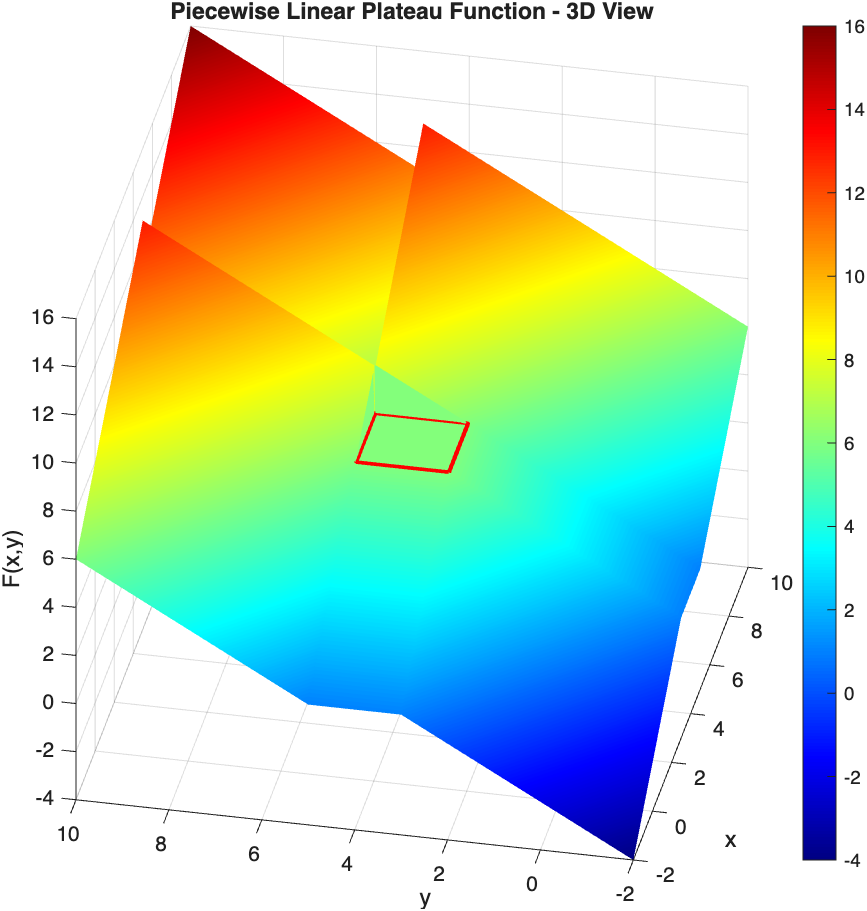
\includegraphics[width=0.78\textwidth]{PiecewiseLinearPlateauPlot.png}
\caption{Graf funkcije \texttt{PiecewiseLinearPlateau}.}
\label{fig:piecewise-plot}
\end{figure}

Na sliki~\ref{fig:piecewise-basins} je razvidno, da kosovno linearni prehodi ustvarijo izrazite meje, plato pa nastopa kot posebna ravna regija znotraj delitve prostora.

\begin{figure}[htbp]
\centering
\includegraphics[width=0.78\textwidth]{PiecewiseLinearPlateau.png}
\caption{Atrakcijski bazeni funkcije \texttt{PiecewiseLinearPlateau}.}
\label{fig:piecewise-basins}
\end{figure}

Slika~\ref{fig:piecewise-plateaus} potrdi zaznavo glavnega kvadratnega platoja. Ker ima plato veliko notranjih celic, ga jedrni kriterij robustno ohrani.

\begin{figure}[htbp]
\centering
\includegraphics[width=0.78\textwidth]{PiecewiseLinearPlateau_plateaus.png}
\caption{Zaznani platoji funkcije \texttt{PiecewiseLinearPlateau}.}
\label{fig:piecewise-plateaus}
\end{figure}

\subsection{\texttt{TanhRadialStep}}

Funkcija \texttt{TanhRadialStep} je gladka radialna stopnica oziroma vdolbina, določena z razdaljo od izhodišča. Pri privzetih parametrih \(h=10\), \(k=2\) in \(r=3\) je definirana kot
\[
f(x,y)=-\frac{h}{2}\left(1-\tanh\left(k\left(\sqrt{x^2+y^2}-r\right)\right)\right).
\]
Slika~\ref{fig:tanh-plot} prikazuje gladek prehod iz globlje centralne regije proti zunanji skoraj ravni površini.

\begin{figure}[htbp]
\centering
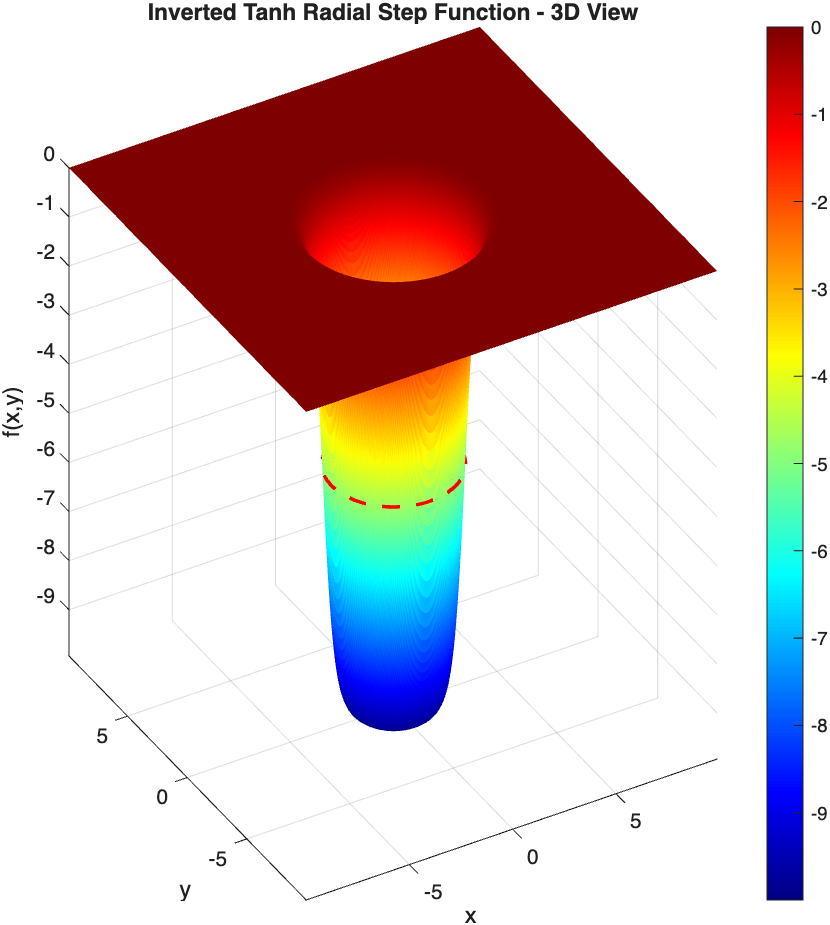
\includegraphics[width=0.78\textwidth]{TanhRadialStepPlot.png}
\caption{Graf funkcije \texttt{TanhRadialStep}.}
\label{fig:tanh-plot}
\end{figure}

Na sliki~\ref{fig:tanh-basins} se pokaže radialna struktura funkcije. Ker funkcija nima eksplicitno definiranega platoja z natančno konstantno vrednostjo, so meje in regije močno odvisne od vzorčenja in numerične predstavitve vrednosti.

\begin{figure}[htbp]
\centering
\includegraphics[width=0.78\textwidth]{TanhRadialStep.png}
\caption{Atrakcijski bazeni funkcije \texttt{TanhRadialStep}.}
\label{fig:tanh-basins}
\end{figure}

Slika~\ref{fig:tanh-plateaus} je pomembna kot prikaz omejitve metode. Zaznane ravne regije pri tej funkciji niso nujno pravi analitični platoji, temveč so lahko posledica zelo postopnega padca funkcije, končne ločljivosti mreže in zaokroževanja vrednosti pri računanju. To pomeni, da diskretni algoritem lahko najde navidezne platoje tam, kjer je zvezna funkcija le zelo položna. Primer zato kaže, da je treba rezultate pri gladkih funkcijah interpretirati skupaj z obliko funkcije in po potrebi uvesti dodatne kriterije, na primer toleranco, lokalno varianco ali preverjanje gradienta.

\begin{figure}[htbp]
\centering
\includegraphics[width=0.78\textwidth]{TanhRadialStep_plateaus.png}
\caption{Zaznani platoji funkcije \texttt{TanhRadialStep}; ti lahko predstavljajo diskretizacijske artefakte in ne pravih analitičnih platojev.}
\label{fig:tanh-plateaus}
\end{figure}

\section{Razprava}

Glavna prednost razširitve je, da obstoječi cevovod za atrakcijske bazene ni bil zamenjan, temveč nadgrajen. Meje med bazeni se še vedno določijo pred barvanjem, dodatni pogoji v \texttt{makeBoundariesPlateau} pa omogočijo, da se upoštevajo tudi prehodi v ravna območja. Zaznavanje platojev je izvedeno po barvanju bazenov, zato lahko sistem za vsako celico hrani tako informacijo o bazenu kot informacijo o platoju.

Pomembna odločitev je uporaba jedra regije namesto same velikosti regije. Ta odločitev neposredno naslovi problem lažno pozitivnih zaznav, saj enopikselske črte in posamezne točke nimajo notranjosti. Metoda zato bolje ustreza intuitivni predstavi platoja kot dvodimenzionalnega ravnega območja.

Omejitev pristopa je, da primerjava vrednosti funkcije trenutno temelji na natančni enakosti tipa \texttt{double}. To je primerno za funkcije, kjer so platoji ustvarjeni z eksplicitnim prirejanjem iste vrednosti, na primer z odrezom funkcije ali kosovno definicijo. Pri funkcijah, kjer zaradi numeričnega šuma vrednosti na platoju niso popolnoma enake, bi bilo smiselno dodati toleranco \(\varepsilon\), tako da bi celici obravnavali kot enaki, kadar velja
\[
|f_a - f_b| \le \varepsilon.
\]

Druga omejitev je odvisnost od ločljivosti mreže. Plato, ki je v zveznem prostoru majhen, je lahko pri prenizki ločljivosti vzorčen le kot nekaj pik ali črta in bo zato pravilno zavrnjen glede na diskretno sliko, čeprav v zvezni funkciji obstaja. Zato je izbira ločljivosti in parametra \texttt{minPlateauSize} del metodološke nastavitve eksperimenta.

\section{Zaključek}

V nalogi je bila obstoječa analiza atrakcijskih bazenov razširjena z zaznavanjem platojev in mej med platoji ter bazeni. Razširitev vključuje dopolnjeno zaznavanje mej, novo funkcijo \texttt{detectPlateaus}, filtriranje majhnih in pretankih regij z jedrom po 4-sosedstvu ter ločen izris platojev v razredu \texttt{Measure}. S tem je analiza bolj primerna za optimizacijske funkcije, ki vsebujejo ravna območja in pri katerih samo barvanje atrakcijskih bazenov ne poda celotne slike strukture iskalnega prostora.

Nadaljnje delo lahko vključuje eksperimentalno primerjavo na več testnih funkcijah, uvedbo tolerance za primerjavo vrednosti funkcije, kvantitativno poročanje o velikostih platojev in povezavo zaznanih platojev z obnašanjem izbranih optimizacijskih algoritmov.

\begin{thebibliography}{1}

\bibitem{jerebic_novel_2021}
J. Jerebic, M. Mernik, S.-H. Liu, M. Ravber, M. Baketarić, L. Mernik, and M. Črepinšek, ``A novel direct measure of exploration and exploitation based on attraction basins,'' \emph{Expert Systems with Applications}, vol. 167, p. 114353, Apr. 2021, doi: 10.1016/j.eswa.2020.114353.

\end{thebibliography}

\end{document}
